\section{Theory}
\paragraph{Gamma radiation?}

\paragraph{Scintillation detector}
Scintillation detectors are based on the properties of \emph{scintillators}, 
materials that emit photons in the visible spectrum after the passage of a charged particle.
The scintillators used for particle detection are primarily [split] between two types: 
organic (or plastic), in which the photon emission has molecular origin, 
and inorganic (or crystalline), crystals which are doped with activators that can first be excited by electron-hole pairs 
produced by the charged particle passing in the crystal lattice and then deexcite by photon emission \cite{intro_nuclear_particle_physics}.

\begin{figure}[htbp]
    \centering
    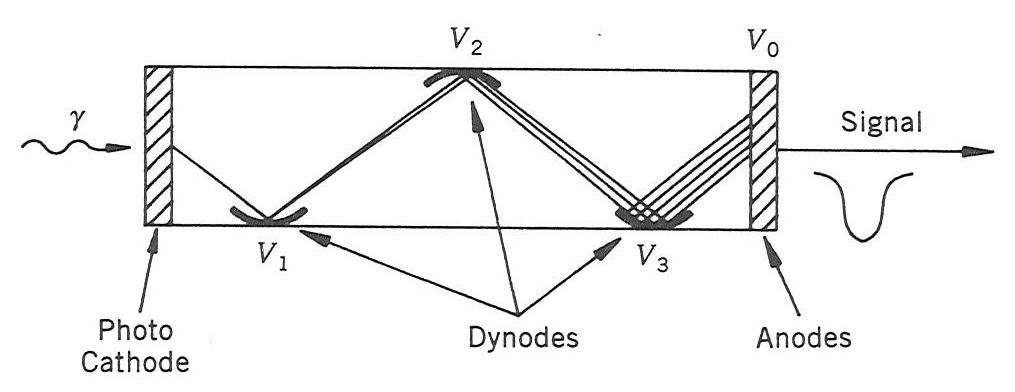
\includegraphics[scale=1]{figures/photomultiplier.jpg}
    \caption{Main elements of a photomultiplier tube \cite{intro_nuclear_particle_physics}.}
    \label{fig:photomultiplier}
\end{figure}

\paragraph{Gamma spectrometry}
[Expliquer l'apparition d'une gaussienne à la place d'une ligne pour les peaks des spectres]


\paragraph{Experimental setup}
[? dire que on utilise inorganic?]